\documentclass[usenames, dvipsnames, aspectratio=169]{beamer}

%%%%%
%%%%%
%%%%%
%%%%%
%%%%%

\usepackage{xcolor}
\usepackage{tikz}
\usetikzlibrary{backgrounds}
\usetikzlibrary{arrows, shapes}
\usetikzlibrary{tikzmark}
\usetikzlibrary{calc}
\usetikzlibrary{positioning}
\usetikzlibrary{shadows}
\usetikzlibrary{trees, mindmap}

\usepackage{pgfplots}
\pgfplotsset{compat=newest}

\usepackage{tcolorbox}

\newcommand{\highlight}[2]{\colorbox{#1!17}{$\displaystyle #2$}}
\newcommand{\highlightdark}[2]{\colorbox{#1!47}{$\displaystyle #2$}}
\renewcommand{\highlight}[2]{\colorbox{#1!17}{#2}}
\renewcommand{\highlightdark}[2]{\colorbox{#1!47}{#2}}

\usepackage[utf8]{inputenc}
\usepackage[english]{babel}

\usepackage{amsmath, amssymb, amsfonts}

\usepackage[]{bm}
\usepackage[]{nicefrac}

\usepackage{graphicx}
\usepackage{multimedia}

\usepackage{xspace}

\newcommand{\lap}{\nabla^2}

%%%%%
%%%%%
%%%%%
%%%%%
%%%%%





\usetheme{default}
\usefonttheme{professionalfonts}
\setbeamertemplate{navigation symbols}{}
\setbeamertemplate{itemize items}[circle]
\setbeamercolor{itemize item}{fg=white}

\setbeamerfont{title}{series=\bfseries, size=\normalfont\Large}
\setbeamercolor{title}{fg=white}

\setbeamerfont{author}{size=\normalfont\small}
\setbeamercolor{author}{fg=white}

\setbeamerfont{frametitle}{series=\bfseries, size=\normalfont}
\setbeamercolor{frametitle}{fg=white}

\setbeamerfont{framesubtitle}{size=\normalfont\large}
\setbeamercolor{framesubtitle}{fg=white}

\setbeamercolor{background canvas}{bg=black}
\setbeamercolor{normal text}{fg=white}

\setbeamercolor{local structure}{fg=white}





\graphicspath{{imgs/}}





\title{Lorenz system}
\author{Jean-Christophe LOISEAU}
\institute{Arts \& Métiers Institute of Technology, January 2022}
\date{}

\begin{document}

\frame{\titlepage}

{
  \setbeamercolor{background canvas}{bg=white}
  \setbeamercolor{background canvas}{bg=white}
  \setbeamercolor{normal text}{fg=black}

  \usebeamercolor[fg]{normal text}

  \setbeamercolor{frametitle}{fg=black}
  \setbeamercolor{framesubtitle}{fg=black}
  \setbeamercolor{itemize item}{fg=black}

  \begin{frame}
    \vfill
    \centering
    \large
    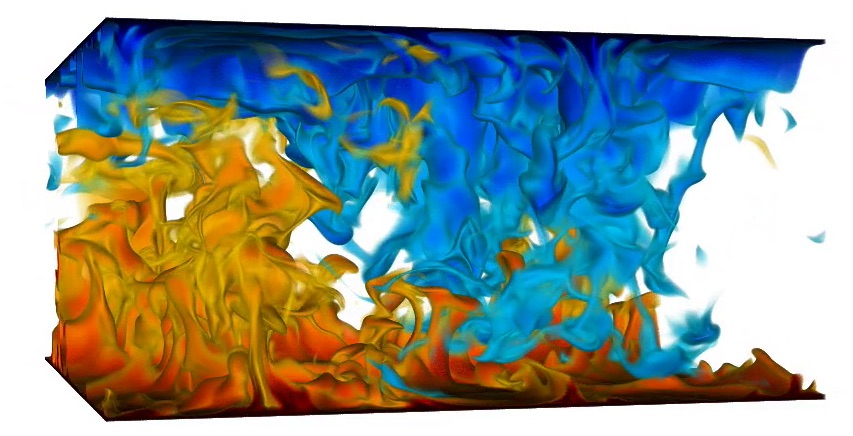
\includegraphics[width=\textwidth]{RB}
    \vfill
  \end{frame}

}



\begin{frame}[t, c, fragile]{Rayleigh-Bénard convection}{Velocity equation}
  \vfill
  \large

  \begin{equation}
    \tikzmarknode{a} {\highlightdark{red}{$\dfrac{\partial \bm{u}}{\partial t}$}}
    +
    \tikzmarknode{b} {\highlightdark{blue}{$\left( \bm{u} \cdot \nabla \right) \bm{u}$}}
    =
    -
    \tikzmarknode{c} {\highlightdark{Plum}{$\dfrac{1}{\rho} \nabla p$}}
    +
    \tikzmarknode{d} {\highlightdark{BlueViolet}{$\nu \lap  \bm{u}$}}
    +
    \tikzmarknode{e} {\highlightdark{PineGreen}{$\delta \rho \bm{g}$}}
    \notag
  \end{equation}
  %
  \begin{tikzpicture}[overlay, remember picture, >=stealth, nodes={align=left, inner ysep=1pt}, <-]
    \path (a.north) ++ (0, 2em) node[anchor=south east, color=red!67] (inertia){Inertia};
    \draw [color=red!87] (a.north) |- ([xshift=0.3ex, color=red] inertia.south west);

    \path (b.south) ++ (0, -2em) node[anchor=north west, color=blue!67] (advection){Advection};
    \draw [color=blue!87] (b.south) |- ([xshift=-0.3ex, color=blue] advection.south east);

    \path (c.north) ++ (0, 2em) node[anchor=south east, color=Plum!67] (pressure){Pressure forces};
    \draw [color=Plum!87] (c.north) |- ([xshift=0.3ex, color=red] pressure.south west);

    \path (d.south) ++ (0, -2em) node[anchor=north west, color=BlueViolet!67] (diffusion){Viscous diffusion};
    \draw [color=BlueViolet!87] (d.south) |- ([xshift=-0.3ex, color=BlueViolet] diffusion.south east);

    \path (e.north) ++ (0, 2em) node[anchor=south east, color=PineGreen!67] (buoyancy){Buoyancy};
    \draw [color=PineGreen!87] (e.north) |- ([xshift=0.3ex, color=redPineGreen] buoyancy.south west);
  \end{tikzpicture}

  \vfill
\end{frame}

\begin{frame}[t, c]{Rayleigh-Bénard convection}{Temperature equation}
  \vfill
  \large

  \begin{equation}
    \tikzmarknode{a} {\highlightdark{red}{$\dfrac{\partial T}{\partial t}$}}
    +
    \tikzmarknode{b} {\highlightdark{PineGreen}{$\left( \bm{u} \cdot \nabla \right) T$}}
    =
    \tikzmarknode{c} {\highlightdark{BlueViolet}{$\kappa \lap  T$}}
    \notag
  \end{equation}
  %
  \begin{tikzpicture}[overlay, remember picture, >=stealth, nodes={align=left, inner ysep=1pt}, <-]

    \path (a.north) ++ (0, 2em) node[anchor=south east, color=red!67] (inertia){Inertia};
    \draw [color=red!87] (a.north) |- ([xshift=0.3ex, color=red] inertia.south west);

    \path (b.south) ++ (0, -2em) node[anchor=north west, color=PineGreen!67] (convection){Convection};
    \draw [color=PineGreen!87] (b.south) |- ([xshift=-0.3ex, color=PineGreen] convection.south east);

    \path (c.north) ++ (0, 2em) node[anchor=south east, color=Plum!67] (conduction){Conduction};
    \draw [color=Plum!87] (c.north) |- ([xshift=0.3ex, color=Plum] conduction.south west);

  \end{tikzpicture}

  \vfill
\end{frame}

\begin{frame}[t, c]{Rayleigh-Bénard convection}{Non-dimensional equations}
  \vfill
  \large

  \begin{equation}
    \begin{aligned}
      \dfrac{\partial \bm{u}}{\partial t}
      +
      \left( \bm{u} \cdot \nabla \right) \bm{u}
      & =
      -
      \nabla p
      +
      \tikzmarknode{a} {\highlightdark{PineGreen}{$Pr$}} \lap \bm{u}
      + \left( \tikzmarknode{b} {\highlightdark{blue}{$Ra$}} \cdot
      \tikzmarknode{c} {\highlightdark{PineGreen}{$Pr$}} \right) \vartheta \bm{e}_y \\
      \dfrac{\partial \vartheta}{\partial t} + \left( \bm{u} \cdot \nabla \right) \vartheta & = \lap \vartheta
    \end{aligned}
    \notag
  \end{equation}
  %
  \begin{tikzpicture}[overlay, remember picture, >=stealth, nodes={align=left, inner ysep=1pt}, <-]

    \path (a.north) ++ (0, 2em) node[anchor=south west, color=PineGreen!67] (prandtl){Prandtl number};
    \draw[<->, color=PineGreen!87] (a.north) -- ++ (0, 0.67) -| node[] {} (c.north);

    \path (b.south) ++ (0, -2em) node[anchor=north west, color=blue!67] (rayleigh){Rayleigh number};
    \draw [color=blue!87] (b.south) |- ([xshift=-0.3ex, color=blue] rayleigh.south east);
  \end{tikzpicture}

  \vfill
\end{frame}

\begin{frame}[t, c]{Rayleigh-Bénard convection}{Base flow}
  \vfill
  \large

  \centering
  \underline{Conducting state}
  \begin{overprint}
    \onslide<1>
    \[
    \left\{
    \begin{aligned}
      \dfrac{d^2 \Theta}{dy^2} & = 0 \\
      \Theta(0) & = 1, \quad \Theta(1) = 0
    \end{aligned}
    \right.
    \]
    
    \onslide<2>
    \[
    \begin{aligned}
      \Theta(y) & = 1 - y \\
      \bm{U}_b & = 0
    \end{aligned}
    \]
  \end{overprint}
  \vfill
\end{frame}

\begin{frame}[t, c]{Rayleigh-Bénard convection}{Linear stability}
  \vfill
  \large

  \underline{\textbf{Squire theorem :}} Only two-dimensional perturbations need to be considered.

  \bigskip

  \[
  \begin{aligned}
    \dfrac{\partial \bm{u}^{\prime}}{\partial t} & = -\nabla p^{\prime} + Pr \lap \bm{u}^{\prime} + \left(Ra \cdot Pr \right) \vartheta^{\prime} \bm{e}_y \\
    \dfrac{\partial \vartheta^{\prime}}{\partial t} & = - v^{\prime} + \lap \vartheta^{\prime}
  \end{aligned}
  \]

  \bigskip

  with $\bm{u}^{\prime} = \begin{bmatrix} u^{\prime} & v^{\prime} \end{bmatrix}^T$ and $\vartheta^{\prime}$ the velocity and temperature fluctuations, respectively.
  \vfill
\end{frame}


\begin{frame}[t, c]{Rayleigh-Bénard convection}{Linear stability}
  \vfill
  \large

  \[
  \begin{aligned}
    \dfrac{\partial}{\partial t} \lap \tikzmarknode{a} {\highlightdark{blue}{$\Psi$}} & = - \left( Ra \cdot Pr \right) \dfrac{\partial \vartheta}{\partial x} + Pr \nabla^4 \tikzmarknode{b} {\highlightdark{blue}{$\Psi$}} \\
    \dfrac{\partial \vartheta}{\partial t} & = -\dfrac{\partial \highlightdark{blue}{$\Psi$}}{\partial x} + \lap \vartheta
  \end{aligned}
  \]
  %
  \begin{tikzpicture}[overlay, remember picture, >=stealth, nodes={align=left, inner ysep=1pt}, <-]

    \path (a.north) ++ (0, 2em) node[anchor=south west, color=blue!67] (stream){Fluctuation's streamfunction};
    \draw[<->, color=blue!87] (a.north) -- ++ (0, 0.67) -| node[] {} (b.north);
  \end{tikzpicture}

  \vfill
\end{frame}

\begin{frame}[t, c]{Rayleigh-Bénard convection}{Dispersion relation}
  (1916) Assuming free-slip boundary conditions for the fluctuation leads to

  \[
  \begin{aligned}
    \Psi(x, y, t) & =  \hat{\Psi}(t) \sin(n \pi y) \sin(kx), \\
    \vartheta(x, y, t) & = \hat{\vartheta}(t) \sin(n \pi y) \cos(kx),
  \end{aligned}
  \]

  \bigskip

  the problem can be solved analytically.
  We'll also let $\gamma^2 = \left(n \pi \right)^2 + k^2$.
\end{frame}

\begin{frame}[t, c]{Rayleigh-Bénard convection}{Dispersion relation}
  \vfill
  \large

  \[
  \begin{aligned}
    -\gamma^2 \dfrac{d\hat{\Psi}}{dt} & = Pr \gamma^4 \hat{\Psi} + \left( Ra \cdot Pr \right) k \hat{\vartheta} \\
    \dfrac{d\hat{\vartheta}}{dt} & = -k \hat{\Psi} - \gamma^2 \hat{\vartheta}
  \end{aligned}
  \]

  \vfill
\end{frame}


\begin{frame}[t, c]{Rayleigh-Bénard convection}{Dispersion relation}
  \vfill
  \large

  \[
  \begin{bmatrix}
    -\gamma^2 & 0 \\
    0 & 1
  \end{bmatrix}
  \dfrac{d}{dt}
  \begin{bmatrix}
    \hat{\Psi} \\ \hat{\vartheta}
  \end{bmatrix}
  =
  \begin{bmatrix}
    Pr \gamma^4 & \left( Ra \cdot Pr \right) k \\
    -k & -\gamma^2
  \end{bmatrix}
  \begin{bmatrix}
    \hat{\Psi} \\ \hat{\vartheta}
  \end{bmatrix}
  \]

  \vfill
\end{frame}

\begin{frame}[t, c]{Rayleigh-Bénard convection}{Dispersion relation}
  \vfill
  \large

  \[
  \lambda
  \begin{bmatrix}
    -\gamma^2 & 0 \\
    0 & 1
  \end{bmatrix}
  \begin{bmatrix}
    \hat{\Psi} \\ \hat{\vartheta}
  \end{bmatrix}
  =
  \begin{bmatrix}
    Pr \gamma^4 & \left( Ra \cdot Pr \right) k \\
    -k & -\gamma^2
  \end{bmatrix}
  \begin{bmatrix}
    \hat{\Psi} \\ \hat{\vartheta}
  \end{bmatrix}
  \]

  \vfill
\end{frame}

\begin{frame}[t, c]{Rayleigh-Bénard convection}{Dispersion relation}
  \vfill
  \large

  \begin{minipage}{.48\textwidth}
    \centering
    \underline{Neutral curve}

    \[
    Ra_c(n, k) = \dfrac{\left( \left(n\pi\right)^2 + k^2 \right)^3}{k^2}
    \]
  \end{minipage}%
  \hfill
  \begin{minipage}{.48\textwidth}
    \centering
    \begin{tikzpicture}[>=stealth]
      \begin{axis}[
          xmin=0, xmax=8,
          ymin=0, ymax=2000,
          restrict y to domain=0:2000,
          width=\textwidth,
          samples=4096,
          axis lines = middle,
          axis line style = {->},
          no markers,
          ytick style={draw=none},
          yticklabels=\empty,
          xtick style={draw=none},
          xticklabels=\empty,
          xlabel={Wavenumber $k$}, ylabel={Rayleigh number},
          x label style={at={(axis description cs:0.5,-0.1)},anchor=north},
          y label style={at={(axis description cs:-0.075,.5)},rotate=90,anchor=south},
        ]

        \addplot[domain=0:6, color=orange, ultra thick] {(pi^2 + x^2)^3 / x^2};

        \draw[dashed] (axis cs:0, 657.5) -- (axis cs: 2.22144, 657.5) node[below right] {\tiny $\left( \dfrac{\pi}{2}, \dfrac{27 \pi^4}{4} \right)$};
        \draw[dashed] (axis cs:2.22144, 0) -- (axis cs: 2.22144, 657.5) node[] {};

      \end{axis}
    \end{tikzpicture}
  \end{minipage}

  \vfill
\end{frame}

{
  \setbeamercolor{background canvas}{bg=white}
  \setbeamercolor{background canvas}{bg=white}
  \setbeamercolor{normal text}{fg=black}

  \usebeamercolor[fg]{normal text}

  \setbeamercolor{frametitle}{fg=black}
  \setbeamercolor{framesubtitle}{fg=black}
  \setbeamercolor{itemize item}{fg=black}

  \begin{frame}
    \vfill
    \centering
    \large
    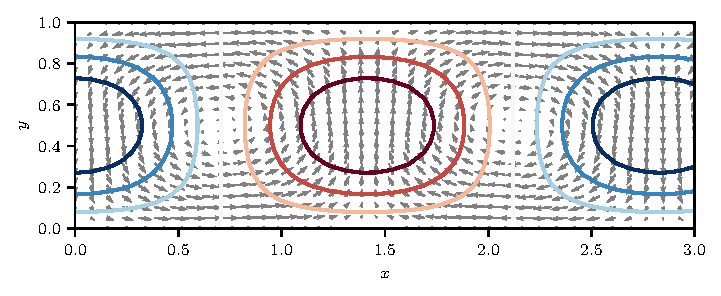
\includegraphics[width=.9\textwidth]{rayleigh_benard_instability_mode}

    Temperature and velocity field of the most unstable eigenmode.
    \vfill
  \end{frame}

}

{
  \setbeamercolor{background canvas}{bg=white}
  \setbeamercolor{background canvas}{bg=white}
  \setbeamercolor{normal text}{fg=black}

  \usebeamercolor[fg]{normal text}

  \setbeamercolor{frametitle}{fg=black}
  \setbeamercolor{framesubtitle}{fg=black}
  \setbeamercolor{itemize item}{fg=black}

  \begin{frame}
    \vfill
    \Large
    \centering

    \textbf{From Navier-Stokes to Lorenz}

    \bigskip

    \large
    \textbf{\color{gray} Investigating the nonlinearities}

    \vfill
  \end{frame}

}

\begin{frame}[t, c]{From Navier-Stokes to Lorenz}{Nonlinear equations}
  \vfill
  \large


  \[
  \begin{aligned}
    \dfrac{\partial}{\partial t} \lap \Psi & = - \left( Ra \cdot Pr \right) \dfrac{\partial \vartheta}{\partial x} + Pr \nabla^4 \Psi
    +
    \tikzmarknode{a} {\highlightdark{blue}{$\mathcal{J}\left[ \lap \Psi, \Psi \right]$}}
    \\
    \dfrac{\partial \vartheta}{\partial t} & = -\dfrac{\partial \Psi}{\partial x} + \lap \vartheta
    +
    \tikzmarknode{b} {\highlightdark{red}{$\mathcal{J}\left[ \vartheta, \Psi \right]$}}
  \end{aligned}
  \]
  %
  \begin{tikzpicture}[overlay, remember picture, >=stealth, nodes={align=left, inner ysep=1pt}, <-]
    \path (a.north) ++ (0, 2em) node[anchor=south east, color=blue!67] (advection){Nonlinear advection};
    \draw [color=blue!87] (a.north) |- ([xshift=0.3ex, color=blue] advection.south west);

    \path (b.south) ++ (0, -2em) node[anchor=south east, color=red!67] (temperature){Nonlinear convection};
    \draw [color=red!87] (b.south) |- ([xshift=0.3ex, color=red] temperature.south west);
  \end{tikzpicture}

  \vfill
\end{frame}

\begin{frame}[t, c]{From Navier-Stokes to Lorenz}{Nonlinear equations}
  \vfill
  \large

  \[
  \mathcal{J}\left[ f, g \right] = \dfrac{\partial f}{\partial x} \dfrac{\partial g}{\partial y} - \dfrac{\partial g}{\partial x} \dfrac{\partial f}{\partial y}
  \]

  \vfill
\end{frame}

\begin{frame}[t, c]{From Navier-Stokes to Lorenz}{Nonlinear equations}
  \vfill
  \large

  \underline{\textbf{Saltzmann} (1962):} The general solution to the partial differential equation can be expressed as a doubly infinite Fourier series

  \vfill
\end{frame}

\begin{frame}[t, c]{From Navier-Stokes to Lorenz}{Deriving the reduced-order model}
  \vfill
  \large

  Close to the bifurcation point, the fluctuations are described by the unstable mode, hence

  \[
  \begin{aligned}
    \Psi(x, y, t) & \simeq \Psi_1(t) \sin(\pi y) \sin(kx) + \cdots \\
    \vartheta(x, y, t) & \simeq \vartheta_1(t) \sin(\pi y) \cos(kx) + \cdots
  \end{aligned}
  \]

  \bigskip

  Which kind of harmonics to they generate due to the nonlinearity ?

  \vfill
\end{frame}

\begin{frame}[t, c]{From Navier-Stokes to Lorenz}{Deriving the reduced-order model}
  \vfill
  \large

  \[
  \begin{aligned}
    \mathcal{J} \left[ \Psi, \lap \Psi \right] & = \mathcal{J} \left[ \Psi, -\gamma^2 \Psi \right] \\
    & = -\gamma^2 \mathcal{J} \left[ \Psi, \Psi \right] \\
    & = 0
  \end{aligned}
  \]

  \vfill
\end{frame}

\begin{frame}[t, c]{From Navier-Stokes to Lorenz}{Deriving the reduced-order model}
  \vfill
  \large

  \[
  \begin{aligned}
    \mathcal{J} \left[ \Psi, \vartheta \right] & = \Psi_1 \vartheta_1 \mathcal{J} \left[ \sin(kx) \sin(\pi y), \sin(kx) \cos(\pi y) \right] \\
    & = \Psi_1 \vartheta_1 \dfrac{k \pi}{2} \sin( 2\pi y)
  \end{aligned}
  \]

  \vfill
\end{frame}

\begin{frame}[t, c]{From Navier-Stokes to Lorenz}{Deriving the reduced-order model}
  \vfill
  \large

  \[
  \begin{aligned}
    \Psi(x, y, t) & \simeq \tikzmarknode{a} {\highlightdark{blue}{$\Psi_1(t) \sin(kx) \sin(\pi y)$}} \\
    \vartheta(x, y, t) & \simeq {\highlightdark{blue}{$\vartheta_1(t) \sin(kx) \cos(\pi y)$}} + \tikzmarknode{b} {\highlightdark{red}{$\vartheta_2 \sin(2\pi y)$}}
  \end{aligned}
  \]
  %
  \begin{tikzpicture}[overlay, remember picture, >=stealth, nodes={align=left, inner ysep=1pt}, <-]
    \path (a.north) ++ (0, 2em) node[anchor=south east, color=blue!67] (eigenmode){Unstable eigenmode};
    \draw [color=blue!87] (a.north) |- ([xshift=0.3ex, color=blue] eigenmode.south west);
    
    \path (b.south) ++ (0, -2em) node[anchor=north west, color=red!67] (advection){Nonlinear distortion};
    \draw [color=red!87] (b.south) |- ([xshift=-0.3ex, color=red] advection.south east);
  \end{tikzpicture}

  \vfill
\end{frame}

\begin{frame}[t, c]{From Navier-Stokes to Lorenz}{Deriving the reduced-order model}
  \vfill
  \large

  \[
  \dfrac{\partial}{\partial t} \lap \Psi = -\tikzmarknode{a} {\highlightdark{red}{$\left( Ra \cdot Pr \right) \dfrac{\partial \vartheta}{\partial x}$}} + \tikzmarknode{b} {\highlightdark{blue}{$Pr \nabla^4 \Psi$}}
  \]
  %
  \begin{tikzpicture}[overlay, remember picture, >=stealth, nodes={align=left, inner ysep=1pt}, <-]
    \path (a.north) ++ (0, 2em) node[anchor=south east, color=red!67] (buoyancy){Buoyancy};
    \draw [color=red!87] (a.north) |- ([xshift=0.3ex, color=red] buoyancy.south west);
    
    \path (b.south) ++ (0, -3em) node[anchor=south west, color=blue!67] (diffusion){Viscous diffusion};
    \draw [color=blue!87] (b.south) |- ([xshift=0.3ex, color=blue] diffusion.south east);
  \end{tikzpicture}

  \vfill
\end{frame}

\begin{frame}[t, c]{From Navier-Stokes to Lorenz}{Deriving the reduced-order model}
  \vfill
  \large

  \[
  \dfrac{d \Psi_1}{dt} = -\dfrac{k}{\gamma^2} \left( Ra \cdot Pr \right) \vartheta_1 - Pr \gamma^2 \Psi_1
  \]

  \vfill
\end{frame}

\begin{frame}[t, c]{From Navier-Stokes to Lorenz}{Deriving the reduced-order model}
  \vfill
  \large

  \[
  \dfrac{\partial \vartheta}{\partial t} = -\tikzmarknode{a} {\highlightdark{red}{$\dfrac{\partial \Psi}{\partial x}$}} + \tikzmarknode{b} {\highlightdark{blue}{$\lap \vartheta$}} + \tikzmarknode{c} {\highlightdark{PineGreen}{$\mathcal{J}\left[ \vartheta, \Psi \right]$}}
  \]
  %
  \begin{tikzpicture}[overlay, remember picture, >=stealth, nodes={align=left, inner ysep=1pt}, <-]
    \path (a.north) ++ (0, 2em) node[anchor=south east, color=red!67] (convection){Convection};
    \draw [color=red!87] (a.north) |- ([xshift=0.3ex, color=red] convection.south west);
    
    \path (b.south) ++ (0, -3em) node[anchor=south west, color=blue!67] (diffusion){Thermal diffusion};
    \draw [color=blue!87] (b.south) |- ([xshift=0.3ex, color=blue] diffusion.south east);

    \path (c.north) ++ (0, 2em) node[anchor=south west, color=PineGreen!67] (distortion){Nonlinear distortion};
    \draw [color=PineGreen!87] (c.north) |- ([xshift=0.3ex, color=red] distortion.south east);
  \end{tikzpicture}

  \vfill
\end{frame}

\begin{frame}[t, c]{From Navier-Stokes to Lorenz}{Deriving the reduced-order model}
  \vfill
  \large

  \[
  \begin{aligned}
    \dfrac{d \vartheta_1}{dt} & = k \Psi_1 \left( 1 + \pi \vartheta_2 \right) - \gamma^2 \vartheta_1 \\
    \dfrac{d \vartheta_2}{dt} & = \dfrac{k\pi}{2} \Psi_1 \vartheta_1 - 4\pi^2 \vartheta_2
  \end{aligned}
  \]

  \vfill
\end{frame}

\begin{frame}[t, c]{From Navier-Stokes to Lorenz}{Deriving the reduced-order model}
  \vfill
  \large

  \[
  \begin{aligned}
    \dfrac{d \Psi_1}{dt} & = \dfrac{k}{\gamma^2} \left( Ra \cdot Pr \right) \vartheta_1 - Pr \gamma^2 \Psi_1 \\
    \dfrac{d \vartheta_1}{dt} & = \Psi_1 \left( k + k \pi \vartheta_2 \right) - \gamma^2 \vartheta_1 \\
    \dfrac{d \vartheta_2}{dt} & = \dfrac{k\pi}{2} \Psi_1 \vartheta_1 - 4\pi^2 \vartheta_2
  \end{aligned}
  \]

  \vfill
\end{frame}

\begin{frame}[t, c]{From Navier-Stokes to Lorenz}{Deriving the reduced-order model}
  \vfill
  \large

  \[
  \begin{aligned}
    \dot{x} & = \sigma \left( y - x \right) \\
    \dot{y} & = x \left( \rho - z \right) - y \\
    \dot{z} & = xy - \beta z
  \end{aligned}
  \]

  \vfill  
\end{frame}

{
  \setbeamercolor{background canvas}{bg=white}
  \setbeamercolor{background canvas}{bg=white}
  \setbeamercolor{normal text}{fg=black}

  \usebeamercolor[fg]{normal text}

  \setbeamercolor{frametitle}{fg=black}
  \setbeamercolor{framesubtitle}{fg=black}
  \setbeamercolor{itemize item}{fg=black}

  \begin{frame}
    \vfill
    \Large
    \centering

    \textbf{Lorenz system}

    \bigskip

    \large
    \textbf{\color{gray} A case study}

    \vfill
  \end{frame}

}

\begin{frame}[t, c]{Lorenz model}{Some fundamental properties}
  \vfill
  \large

  \underline{\textbf{Equivariance} :} The equations remain unchanged if $(x, y, z) \mapsto (-x, -y, z)$.

  \[
  \bm{S} \dot{\bm{x}} = \bm{f}(\bm{Sx})
  \]

  \bigskip

  If $(x, y, z)$ is a solution, so is $(-x, -y, z)$.
  They come in pairs.

  \vfill
\end{frame}

\begin{frame}[t, c]{Lorenz model}{Some fundamental properties}
  \vfill
  \large

  \underline{\textbf{Invariant axis} :} If $x(0) = y(0) = 0$, then $x(t) = y(t) = 0$ at all time.

  \[
  \dot{z} = - \beta z \quad \Rightarrow \quad z(t) = \exp(-\beta t) z_0
  \]

  \bigskip

  The $z$-axis is an \textbf{\alert{invariant manifold}} of the system.

  \vfill
\end{frame}

\begin{frame}[t, c]{Lorenz model}{Some fundamental properties}
  \vfill
  \large

  \underline{\textbf{Strongly dissipative} :} Every in phase space, we have that

  \[
  \nabla \cdot \bm{f}(\bm{x}) = -\sigma - 1 - \beta < 0.
  \]

  \bigskip

  Any given volume $V$ of initial conditions will eventually tend to 0 as $t \to \infty$.

  \vfill
\end{frame}

\begin{frame}[t, c]{Lorenz model}{Exercise}
  \vfill
  \large

  \begin{minipage}{.68\textwidth}
    \underline{\textbf{Exercise}} : Onset of the convection cells

    \bigskip

    \begin{enumerate}
    \item Compute the fixed points of the system as a function of $\rho$.

    \item When does the conducting state ($\bm{x} = 0$) loose its stability?

    \item Using a symmetry argument, what type of bifurcation can it be?
    \end{enumerate}
  \end{minipage}%
  \hfill
  \begin{minipage}{.28\textwidth}
    \[
    \begin{aligned}
      \dot{x} & = \sigma \left( y - x \right) \\
      \dot{y} & = x \left( \rho - z \right) - y \\
      \dot{z} & = xy - \beta z
    \end{aligned}
    \]
  \end{minipage}

  \vfill
\end{frame}
{
  \setbeamercolor{background canvas}{bg=white}
  \setbeamercolor{background canvas}{bg=white}
  \setbeamercolor{normal text}{fg=black}

  \usebeamercolor[fg]{normal text}

  \setbeamercolor{frametitle}{fg=black}
  \setbeamercolor{framesubtitle}{fg=black}
  \setbeamercolor{itemize item}{fg=black}

  \begin{frame}[t, c]{Lorenz system}{Dynamics for $1 \leq \rho \leq 14$}
    \vfill
    \centering
    \large
    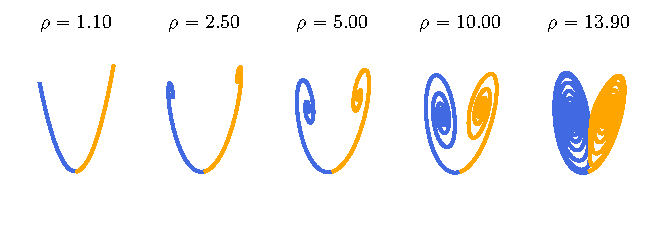
\includegraphics[width=\textwidth]{primary_bifurcation_phase_plots}
    \vfill
  \end{frame}

}

\begin{frame}[t, c]{Lorenz system}{Homoclinic connection ($\rho \simeq 13.926$)}
  \vfill
  \large

  \begin{minipage}{.48\textwidth}
    Perturbation leaves the conducting state along its unstable manifold and returns to it along its stable one.
  \end{minipage}%
  \hfill
  \begin{minipage}{.48\textwidth}
    \centering
    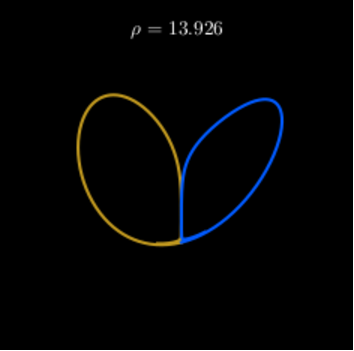
\includegraphics[width=\textwidth]{homoclinic_connection}
  \end{minipage}

  \vfill
\end{frame}

\begin{frame}[t, c]{Lorenz system}{Transient chaos}
  \vfill
  \large
  For $\rho > 14$, the system exhibits \textbf{sensitive dependence on initial conditions}.

  \bigskip

  \begin{tikzpicture}[>=stealth]
    \begin{axis}[
        xmin=0, xmax=50,
        ymin=-30, ymax=30,
        xlabel={Time $t$}, ylabel={$x(t)$},
        width=\textwidth,
        height=.66\textheight,
        axis lines = middle,
        axis line style = {->},
        x label style={at={(axis description cs:0.5, -0.1)}, anchor=north},
        y label style={at={(axis description cs:0, 0.5)}, rotate=90, anchor=south},
        ytick style={draw=none},
        yticklabels=\empty,
        xtick style={draw=none},
        xticklabels=\empty,
      ]

      \addplot[thick, no markers, smooth] table[x=t, y=x]{data/lorenz_transients_trial_1.dat};
      \addplot[thick, no markers, smooth, blue!67] table[x=t, y=x]{data/lorenz_transients_trial_2.dat};
      \addplot[thick, no markers, smooth, red!67] table[x=t, y=x]{data/lorenz_transients_trial_3.dat};

      \draw[white, thin] (axis cs:30, 30) -- (axis cs:48, 48) node[] {};
    \end{axis}
  \end{tikzpicture}

  \vfill
\end{frame}

\begin{frame}[t, c]{Lorenz system}{Strange attractor for $(\sigma, \rho, \beta) = (10, 28, 8/3)$}
  \centering
  \begin{tikzpicture}[>=stealth]
    \begin{axis}[
        xmin=0, xmax=50,
        ymin=0, ymax=50,
        xlabel={$x(t)$}, ylabel={$z(t)$},
        height=.75\textheight,
        axis lines = middle,
        axis line style = {->},
        x label style={at={(axis description cs:1, 0)}, anchor=north},
        y label style={at={(axis description cs:0, 1)}, anchor=west},
        no markers,
        ytick style={draw=none},
        yticklabels=\empty,
        xtick style={draw=none},
        xticklabels=\empty,
      ]
      \addplot[smooth, thin, white] table[x=x, y=z]{data/lorenz_attractor.dat};
    \end{axis}
  \end{tikzpicture}
\end{frame}

\begin{frame}[t, c]{Lorenz system}{Strange attractor}
  \vfill
  \large

  \begin{minipage}{.48\textwidth}
    \begin{overprint}
      \onslide<1>
      The attractor is not a volume, but not a surface either.
      It is something in-between: a \alert{\textbf{fractal object}}.

      \onslide<2>
      Its dimension is estimated to be
      %
      \[
      2.06 \pm 0.01,
      \]
      %
      i.e.\ it is not an integer.
    \end{overprint}
  \end{minipage}%
  \hfill
  \begin{minipage}{.48\textwidth}
    \centering
    \begin{tikzpicture}[>=stealth]
      \begin{axis}[
          xmin=-25, xmax=25,
          ymin=-25, ymax=25,
          xlabel={$x$}, ylabel={$y$},
          width=\textwidth,
          axis lines = middle,
          axis line style = {->},
          x label style={at={(axis description cs:1, 0.5)}, anchor=north},
          y label style={at={(axis description cs:0.5, 1)}, anchor=west},
          ytick style={draw=none},
          yticklabels=\empty,
          xtick style={draw=none},
          xticklabels=\empty,
        ]

        \addplot[only marks, orange, mark size=0.25pt] table[x=x, y=y]{data/poincare_section.dat};

      \end{axis}
    \end{tikzpicture}
  \end{minipage}

  \vfill
\end{frame}

\begin{frame}[t, c]{Lorenz system}{Strange attractor}
  \vfill
  \large

  \[
  t_{\text{horizon}} \sim \mathcal{O} \left( \dfrac{1}{\tikzmarknode{a} {\highlightdark{red}{$\lambda$}}} \log \dfrac{\tikzmarknode{b} {\highlightdark{blue}{$a$}}}{\tikzmarknode{c} {\highlightdark{PineGreen}{$\delta_0$}}} \right)
  \]
  \begin{tikzpicture}[overlay, remember picture, >=stealth, nodes={align=left, inner ysep=1pt}, <-]

    \path (a.south) ++ (0, -2em) node[anchor=south east, color=red!67] (lyapunov){Lyapunov exponent};
    \draw [color=red!87] (a.south) |- ([xshift=0.3ex, color=red] lyapunov.south west);

    \path (b.north) ++ (0, 2em) node[anchor=south west, color=blue!67] (accuracy){Accuracy of the prediction};
    \draw [color=blue!87] (b.north) |- ([xshift=-0.3ex, color=blue] accuracy.south east);

    \path (c.south) ++ (0, -5em) node[anchor=south east, color=PineGreen!67] (uncertainty){Uncertainty on the initial condition};
    \draw [color=PineGreen!87] (c.south) |- ([xshift=0.3ex, color=red] uncertainty.south west);

  \end{tikzpicture}

  \vfill
\end{frame}

\begin{frame}[t, c, fragile]{Lorenz system}{Strange attractor}
  \vfill
  \large

  \[
  t_{\text{Lorenz}} \sim \mathcal{O} \left( \log \dfrac{a}{\delta_0} \right)
  \]

  \vfill
\end{frame}

{
  \setbeamercolor{background canvas}{bg=white}
  \setbeamercolor{background canvas}{bg=white}
  \setbeamercolor{normal text}{fg=black}
  
  \usebeamercolor[fg]{normal text}
  
  \setbeamercolor{frametitle}{fg=black}
  \setbeamercolor{framesubtitle}{fg=black}
  \setbeamercolor{itemize item}{fg=black}
  
  \begin{frame}
    \vfill
    \centering
    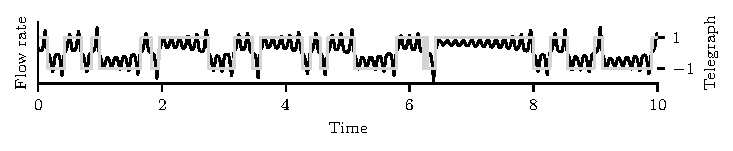
\includegraphics[width=\textwidth]{flow_rate_telegraph_signal}
    
    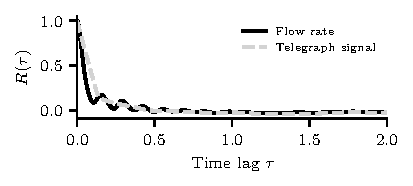
\includegraphics[width=.48\textwidth]{flow_rate_autocorrelation}%
    \hfill
    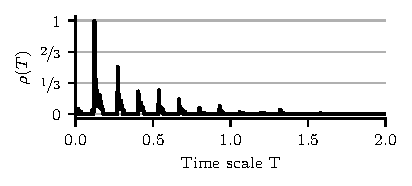
\includegraphics[width=.48\textwidth]{flow_rate_time_scale_distribution}

    \vfill
  \end{frame}

}

\begin{frame}[t, c]{Lorenz system}{Strange attractor}
  \begin{tikzpicture}[>=stealth]
    \begin{axis}[
        xmin=0, xmax=30,
        ymin=0, ymax=50,
        xlabel={Time $t$}, ylabel={$z(t)$},
        width=\textwidth,
        height=.5\textheight,
        axis lines = middle,
        axis line style = {->},
        x label style={at={(axis description cs:0.5, -0.1)}, anchor=north},
        y label style={at={(axis description cs:0, 0.5)}, rotate=90, anchor=south},
        ytick style={draw=none},
        yticklabels=\empty,
        xtick style={draw=none},
        xticklabels=\empty,
      ]

      \addplot[thin, no markers, smooth] table[x=t, y=z]{data/lorenz_z_time_series.dat};
      \addplot[only marks, orange, mark size=1.5pt] table[x=t, y=z]{data/lorenz_events.dat};

      \draw[white, thin] (axis cs:30, 30) -- (axis cs:48, 48) node[] {};
    \end{axis}
  \end{tikzpicture}
\end{frame}

\begin{frame}[t, c]{Lorenz system}{Strange attractor}
  \vfill
  \large

  \begin{minipage}{.48\textwidth}
    \centering
    \underline{\textbf{Lorenz map}}

    \begin{overprint}
      \onslide<1>
      \[
      z_{k+1} = f(z_k)
      \]

      \onslide<2>
      \[
      \vert f^{\prime}(z) \vert > 1 \quad \forall z
      \]
    \end{overprint}
  \end{minipage}%
  \hfill
  \begin{minipage}{.48\textwidth}
    \centering
    \begin{tikzpicture}[>=stealth]
      \begin{axis}[
          xmin=30, xmax=48,
          ymin=30, ymax=48,
          xlabel={$z_k$}, ylabel={$z_{k+1}$},
          width=\textwidth,
          axis lines = middle,
          axis line style = {->},
          x label style={at={(axis description cs:1, 0)}, anchor=north},
          y label style={at={(axis description cs:0, 1)}, anchor=west},
          ytick style={draw=none},
          yticklabels=\empty,
          xtick style={draw=none},
          xticklabels=\empty,
        ]

        \addplot[only marks, orange, mark size=0.5pt] table[x=x, y=y]{data/lorenz_map.dat};

        \draw[white, thin] (axis cs:30, 30) -- (axis cs:48, 48) node[] {};
      \end{axis}
    \end{tikzpicture}
  \end{minipage}

  \vfill
\end{frame}

\begin{frame}[t, c]{Lorenz system}{Strange attractor}
  \vfill
  \large

  \begin{minipage}{.48\textwidth}
    \centering
    \underline{\textbf{Period-2 orbit}}
    \begin{overprint}
      \onslide<1>
      \[
      z = \left( f \circ f \right)(z)
      \]

      \onslide<2>
      \[
      \eta_{k+2} \simeq \left( f^{\prime}(p) f^{\prime}(q) \right) \eta_k
      \]
    \end{overprint}
  \end{minipage}%
  \hfill
  \begin{minipage}{.48\textwidth}
    \centering
    \begin{tikzpicture}[>=stealth]
      \begin{axis}[
          xmin=30, xmax=48,
          ymin=30, ymax=48,
          xlabel={$z_k$}, ylabel={$z_{k+2}$},
          width=\textwidth,
          axis lines = middle,
          axis line style = {->},
          x label style={at={(axis description cs:1, 0)}, anchor=north},
          y label style={at={(axis description cs:0, 1)}, anchor=west},
          ytick style={draw=none},
          yticklabels=\empty,
          xtick style={draw=none},
          xticklabels=\empty,
        ]

        \addplot[only marks, orange, mark size=0.5pt] table[x=x, y=y]{data/lorenz_map_bis.dat};

        \draw[white, thin] (axis cs:30, 30) -- (axis cs:48, 48) node[] {};
      \end{axis}
    \end{tikzpicture}
  \end{minipage}

  \vfill
\end{frame}

\begin{frame}[t, c]{Lorenz system}{Strange attractor}
  \vfill
  \large

  \begin{minipage}{.48\textwidth}
    \centering
    \underline{\textbf{Period-n orbit}}
    \begin{overprint}
      \onslide<1>
      \[
      z = \left( f \circ f \circ \cdots \circ f \right)(z)
      \]

      \onslide<2-3>
      \[
      \eta_{k+1} \simeq \left( \prod_{i=1}^{n} f^{\prime}(z_i) \right) \eta_k
      \]
    \end{overprint}
  \end{minipage}%
  \hfill
  \begin{minipage}{.48\textwidth}
    \begin{overprint}
      \onslide<3>
      The skeleton of the attractor is made of an infinite number of \textbf{unstable periodic orbits}.
    \end{overprint}
  \end{minipage}

  \vfill
\end{frame}

{
  \setbeamercolor{background canvas}{bg=white}
  \setbeamercolor{background canvas}{bg=white}
  \setbeamercolor{normal text}{fg=black}

  \usebeamercolor[fg]{normal text}

  \setbeamercolor{frametitle}{fg=black}
  \setbeamercolor{framesubtitle}{fg=black}
  \setbeamercolor{itemize item}{fg=black}

  \begin{frame}
    \vfill
    \Large
    \centering

    \textbf{On the importance of chaos in Science}

    \bigskip

    \large
    \textbf{\color{gray} A (very) brief history}

    \vfill
  \end{frame}

}

\begin{frame}[t, c]{On the importance of chaos in Science}{The clockwork Universe}

  \hfill
  \begin{minipage}{.48\textwidth}
    \centering
    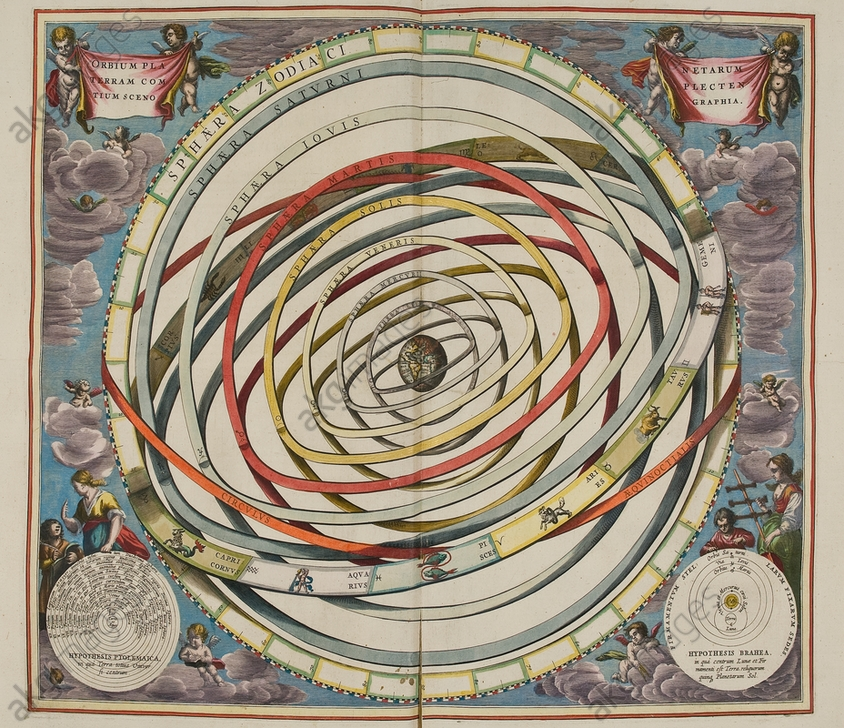
\includegraphics[width=\textwidth]{clockwork}
  \end{minipage}%
  \hfill
  \begin{minipage}{.28\textwidth}
    \centering
    \begin{itemize}
    \item Ptolemy
    \item Copernicus
    \item Gallileo
    \item Kepler
    \item Newton
    \item Leibniz
    \item \ldots
    \end{itemize}
  \end{minipage}
\end{frame}

\begin{frame}[t, c]{On the importance of chaos in Science}{Mathematical determinism}
  \vfill
  \large

  \underline{\textbf{Cauchy-Lipschitz}} (1920): Under suitable regularity conditions on $\bm{f} : \mathbb{R}^n \to \mathbb{R}^n$, the problem

  \[
  \begin{aligned}
    & \dot{\bm{x}} = \bm{f}(\bm{x}) \\
    & \bm{x}(0) = \bm{x}_0
  \end{aligned}
  \]

  \bigskip

  admits a unique solution fully determined by $\bm{f}$ and the initial condition.

  \vfill
\end{frame}

\begin{frame}[t, c]{On the importance of chaos in Science}{Laplace determinism (1814)}
  \vfill
  \large

  \begin{quote}
    Nous devons [...] envisager l'état présent de l'Univers comme l'effet de sont état antérieur, et comme la cause de celui qui va suivre.
    Une intelligence qui pour un instant donné connaîtrait toutes les forces dont la nature est animée et la situation respective des êtes qui la compose [...] embrasserait dans la même formule les mouvements des plus grands corps de l'Univers comme ceux du plus léger atome : rien ne serait incertain pour elle, et l'avenir comme le passé serait présent à ses yeux.
  \end{quote}
  \begin{flushright}
    \emph{Essai philosophie sur les probabilité.}

    Pierre Simon de Laplace, 1814.
  \end{flushright}

  \vfill
\end{frame}

\begin{frame}[t, c]{On the importance of chaos in Science}{The three body problem (circa 1890)}
  \vfill
  \large

  \begin{minipage}{.68\textwidth}
    \centering
    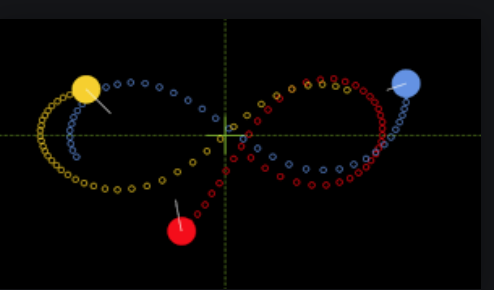
\includegraphics[width=\textwidth]{3body}
  \end{minipage}%
  \hfill
  \begin{minipage}{.28\textwidth}
    \centering
    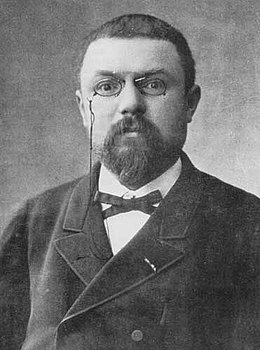
\includegraphics[width=\textwidth]{poincare}
  \end{minipage}

  \vfill
\end{frame}


\begin{frame}[t, c]{On the importance of chaos in Science}{The three body problem (circa 1890)}
  \vfill
  \large

  \begin{quote}
    Si nous connaissions exactement les lois de la nature et la situation de l'univers à l'instant initial, nous pourrions prédire exactement la situation de ce même univers à un instant ultérieur.
    Mais, alors même que les lois naturelles n'auraient plus de secret pour nous, nous ne pourrions connaître la situation qu'approximativement.
    Si cela nous permet de prévoir la situation ultérieure avec la même approximation, c’est tout ce qu’il nous faut, nous disons que le phénomène a été prévu, qu’il est régi par des lois ; mais il n’en est pas toujours ainsi, il peut
    arriver que de petites différences dans les conditions initiales en engendrent de très grandes dans les phénomènes finaux.
  \end{quote}
  \begin{flushright}
    \emph{Calcul des probabilités}

    Henri Poincaré, 1912.
  \end{flushright}

  \vfill
\end{frame}

\begin{frame}[t, c]{On the importance of chaos in Science}{Lorenz (1963)}
  \vfill
  \large
  
  \begin{quote}
    \emph{Chaos: When the present determines the future, but the approximate present does not approximately determine the future.}
  \end{quote}
  %
  \begin{flushright}
    Edward N.\ Lorenz (1917-2008)
  \end{flushright}
  
  \vfill
\end{frame}

{
  \setbeamercolor{background canvas}{bg=white}
  \setbeamercolor{background canvas}{bg=white}
  \setbeamercolor{normal text}{fg=black}

  \usebeamercolor[fg]{normal text}

  \setbeamercolor{frametitle}{fg=black}
  \setbeamercolor{framesubtitle}{fg=black}
  \setbeamercolor{itemize item}{fg=black}

  \begin{frame}[fragile]{}{}
    \vfill
    \flushright
    \Large
    \textbf{\color{black} Thank you for your attention}

    \large
    \textbf{\color{gray} Any question ?}
    \vfill
  \end{frame}
}

\end{document}
